\chapter{Software} \label{Software}
\section{Überblick}
Die Software besteht aus drei unterschiedlichen Teilen mit seperaten Teilaufgaben. Zum einen die Batteriezellenbalancierung und -ladung. Andererseits die eigentliche Motoransteuerung welche per Drathlos-Modul mit dem Magic-Glove(Human Interface) verbunden ist. Das reibungslose Zusammenspiel dieser drei Softwarekomponenten ist äusserst kritisch, da jegliche Softwarefehler extrem gefährlich für den Piloten sein können.
\section{Steuerung - Magic Glove} \label{SW_MagicGlove}
Die Software des Magic-Glove ist um eine einfache Bedienung zu garantieren, sehr simpel aufgebaut. Sie misst in periodischen Abständen von 10ms die Beugung des Fingers des Piloten und übermittelt diesen Wert mittels eingebautem Drahtlos-Modul zur Motorensteuerung, welche die Motordrehzahl entsprechend anpasst. Ausserdem ist es durch Betätigen des Buttons auf der Platine möglich, den Batteriestand des Longboards herauszufinden, welcher dann wiederum auf den 8 angebrachten LED's dargestellt wird. Die Steuerung merkt automatisch wann die Verbindung zum Board verloren ist, stellt diese aber wieder her sobald das Board wieder in Reichweite des Magic Gloves ist.
\section{Stromversorgung} \label{SW_Stromversorgung}
Mit der Software zum Battery Management werden wichtige Punkte geregelt, um ein langes Leben der Akkuzellen zu gewährleisten. Darunter gehören sowohl über- als auch unter- Spannungsschutz sowie ausbalancieren der einzelnen Zellenspannungen beim Laden. \\
Der aktuelle Ladevorgang wird über drei verschiedenen LED’s angezeigt. Dabei zeigen diese den Constant Current (CC), Constant Voltage (CV) und den vollen Zustand (off) an. Diese können als Laden (CC, LED1) Betriebsbereit (CV, LED2) und vollständig geladen (off, LED3) interpretiert werden. 
Das folgende Zustandsdiagramm (Abbildung \ref{fig:statediagrammbatterie}) zeigt den Ablauf der Software auf dem Mikrocontroller.
\begin{figure} [H]
	\centering
	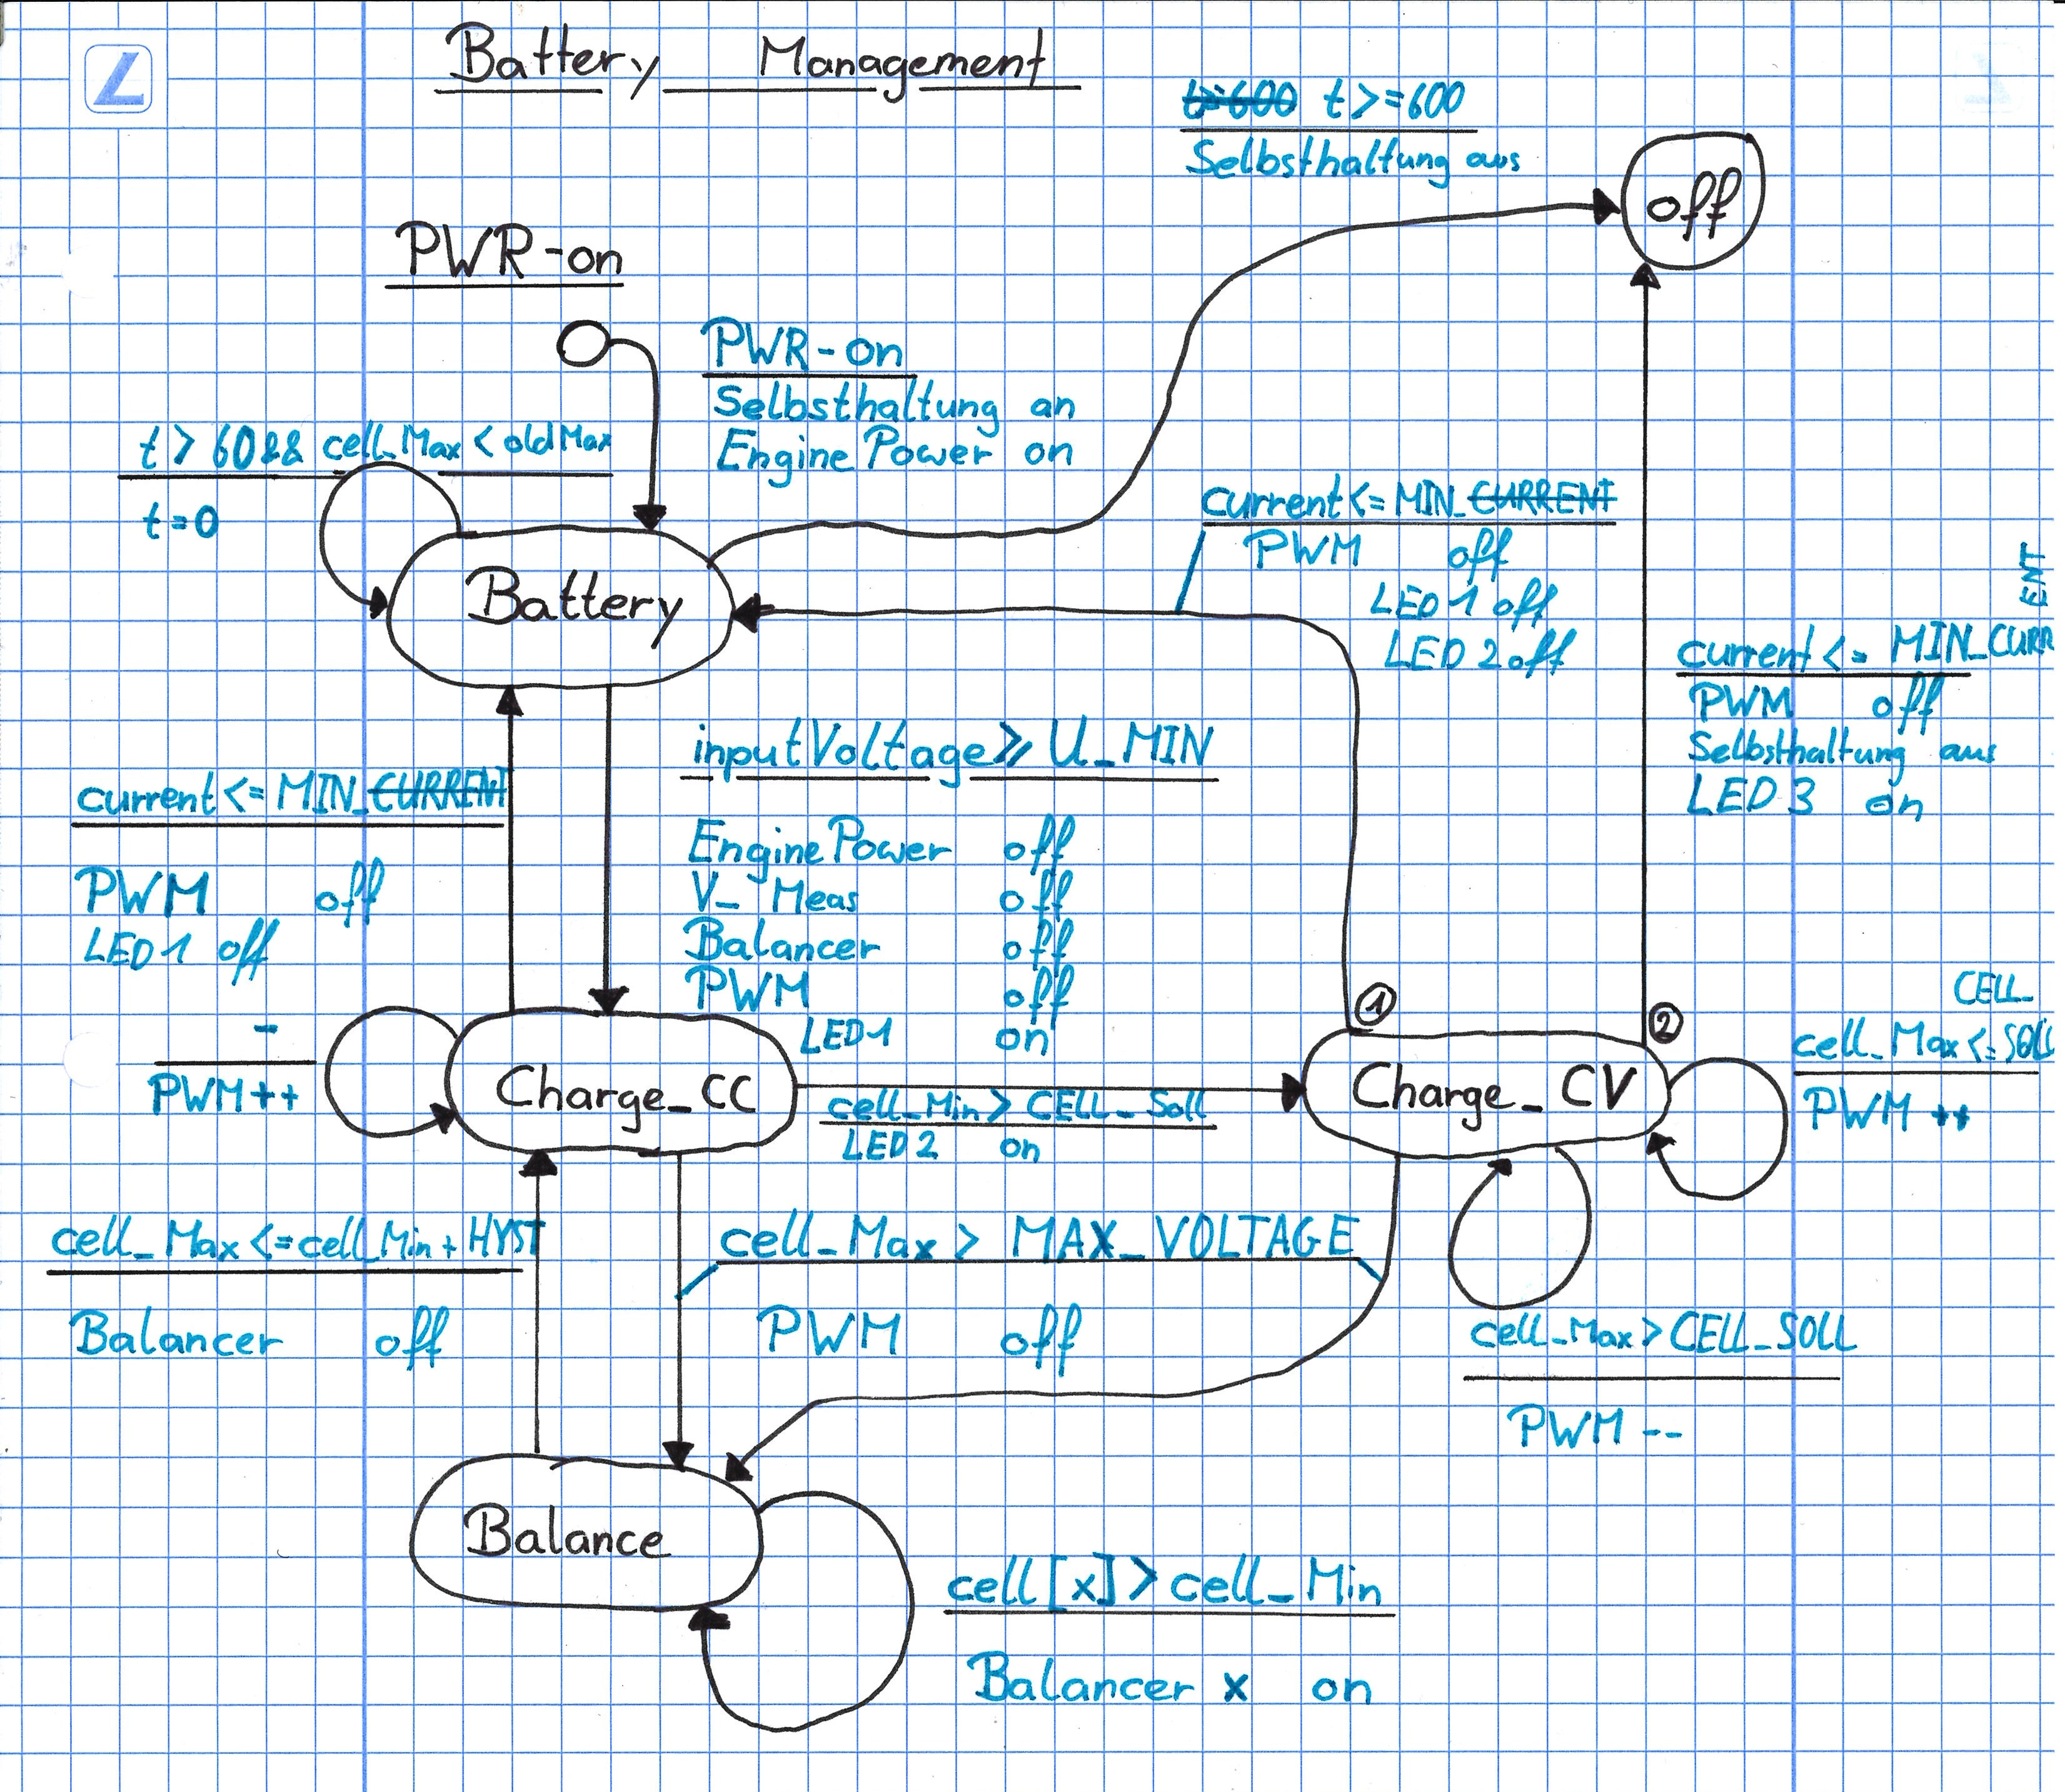
\includegraphics[width=1\linewidth]{images/Statediagramm_Batterie}
	\caption{State Diagramm des Batterie-Management}
	\label{fig:statediagrammbatterie}
\end{figure}
Wie im Hardwareteil schon beschrieben wurde, hält sich der Mikrocontroller mit einer Selbsthaltung in Betrieb. Diese wird jedoch einerseits mit dem Ein- Taster als auch mit der Eingangsspannung des Ladegerätes überbrückt. Wird einer von diesen aktiviert, startet der Mikrocontroller auf und betätigt die Selbsthaltung. \\
Beim Start wird als erstes der \textit{Battery} Zustand geladen. Wenn das Ladekabel nicht angeschlossen ist, wird die Schaltung den Motor mit der benötigten Spannung von den Akkuzellen versorgen. Falls das Board über zehn Minuten nicht gebraucht wird oder sich der Akku der unteren Spannungsgrenze nähert, wird das Board ausgeschaltet. Sobald eine Ladespannung des Ladegeräts angelegt wird, wechselt der Mikrocontroller in den Zustand \textit{Charge\_CC}.\\
In diesem Zustand wird der Strom zunehmend auf die maximalen 5A gebracht und dort konstant gehalten. Dies geschieht durch den Pulsweitenmodulation-Ausgang (PWM-Ausgang) der auf den Schaltregler führt. Je mehr Strom in die Zellen fliesst, desto höher wird deren Spannung. Sobald eine Zelle den Maximalwert von 4.3V überschreitet, wird in den \textit{Balance} Zustand gewechselt. Dort werden alle Zellen auf den Wert der niedrigsten Zelle entladen. Die beiden Zustände werden solange wiederholt, bis sich die  Spannung der niedrigsten Zelle über der Soll Spannung befindet.  Danach wird in den nächsten Zustand \textit{Charge\_CV} gewechselt. \\
Im \textit{Charge\_CV} Zustand wird mit der Regelung des Zuführstromes versucht, die Zellenspannung weiterhin auf dem Sollwert von 4.15V zu halten. Dieser Strom nimmt mit der immer weiter fortschreitenden Aufladung der Zellen kontinuierlich ab, bis schliesslich ein unterer Grenzwert von XXmA \todo{xxx mA} erreicht wird. An diesem Punkt gilt der Akku als voll geladen und wechselt in den Zustand \textit{Off}.
Anders als vielleicht zuerst angenommen bleibt das Board dank der Überbrückung der Selbsthaltung aktiv und zeigt durch die 3 leuchtenden LED’s an, dass der Akku voll aufgeladen ist. Sobald  die Spannung des Ladegeräts abfällt, fällt auch die Selbsthaltung ab. Somit ist das Board komplett ausgeschaltet.
\\\\
Ein weiterer Schwerpunkt der Software war die Berechnung der Spannungen der einzelnen Zellen. Die Zellen sind seriell miteinander verbunden. Somit addieren sich die Spannungen an den Ausgängen jeder Zelle bis auf 24,9V auf der sechsten Zelle. Da der AD-Wandler des Mikrocontroller nur zwischen 0 und 5 Volt messen kann, müssen die Ausgänge der Zellen mit einem Spannungsteiler mit dem Faktor \(\frac 1n\) herunter skaliert werden. Ab der zweiten Spannung sind die Ausgänge jedoch abhängig von den vorherigen Zellen. Um einen richtigen Wert zu erhalten, muss die Differenz inklusive der richtigen Skalierungsfaktoren berechnet werden. Mithilfe dieser Daten kann man für die Spannung der einzelnen Zellen \(cell_0 \dots cell_n\) folgende Formel herleiten:
\begin{equation}
	cell_n = n \cdot ADC(n) - (n-1)\cdot ADC(n-1)
	\label{eq:CellNSpannung}
\end{equation}

\todo{erklärung / Liste der verwendeten Symbole / bedeutung ADC,...}
Die Zellspannungen werden in jedem Durchlauf gemessen und in einem Array abgespeichert. Aus diesen Werten werden die minimale und maximale Spannung berechnet, welche für die verschiedenen Logikabfragen in der Statemachine verwendet werden.

\section{Motoransteuerung} \label{SW_Motoransteuerung}
\subsection*{Plattform}
Zum Einsatz kommt ein STM32F303 Mikrocontroller. Er besitzt eine ARM Cortex-M4 CPU mit FPU und DSP Instruktionen. Als RTOS wird ChibiOS verwendet. Es stellt grundlegende Kernel Funktionalitäten zur Verfügung wie Schedulers und Threads sowie einen HAL. Die komplette Firmware ist in C geschrieben.

Die vom Code generierte Dokumentation kann jederzeit unter \url{https://noah95.github.io/skatemate-sw/} aufgerufen werden.
\subsection*{Entwicklungsumgebung}
\begin{center}
	\begin{tabular}{ | l | l | }
		\hline
		Compiler & arm-none-eabi-gcc 5.4.1 20160919 \\ \hline
		Editor & Sublime Text 3 \\ \hline
		IDE für Debugging & Eclipse CDT \\ \hline
		Debugger Probe & openocd 0.10.0 via ST-Linkv2 \\ \hline
	\end{tabular}
	\captionof{table}{Verwendete SW-Entwicklertools}
\end{center}


\subsection*{Peripherie}
Um dem Microkotroller Rechenleistung abzunehmen werden möglichst viele Aufgaben an die eingebauten Peripheriegeräte ausgelastet. Einige Aufgaben wie das Einlesen von Spannungen kann ausserdem nur von speziellen Peripheriegeräten übernommen werden. In der Tabelle \ref{tab:periph} sind alle verwendeten Peripherien aufgelistet.\\
\begin{tabularx}{\textwidth}{l|c|c|c|X}
	Peripherie & \rotatebox[origin=c]{90}{IRQ} & \rotatebox[origin=c]{90}{DMA} & \rotatebox[origin=c]{90}{DMA IRQ} & Verwendung \\ \hline
	TIM1 &
	- &
	- &
	- &
	Zur Generation der PWM Signale wird der Timer \texttt{TIM1} verwendet. Er ist konfiguriert in Center Aligned PWM Mode. So zählt der Timer zu einem definierten Wert hoch und wieder runter.

	Die PWM Kanäle schalten sobald deren Komperator Wert dem Zählerwert entsprechen. So sind alle PWM ausgänge in der Mitte des Pulses zentriert. Alle Kanäle sind komplementär, so wird der Low-side FET ausgeschaltet wenn der High-side FET eingeschaltet ist und umgekehrt. Kanäle eins bis drei werden für die drei Phasen verwendet und der Kanal vier zur Triggerung des ADC. 

	Der Dutycycle des vierten Kanals ist auf den kleinsten Wert konfiguriert, wo werden die Signale genau in der Mitte des PWM Pulses eingelesen. So wird das \texttt{TIM1 TRGO} Signal generiert.
	\\ \hline
	ADC1 &
	- &
	1 CH1 &
	- &
	Der ADC1 wandelt die drei Phasenspannungen, sowie die Versorgungsspannung. Er wird getriggert von dem \texttt{TIM1 TRGO} Event. Die vier Kanäle werden sequentiell konvertiert und mittels DMA im RAM abgespeichert.
	\\ \hline
	ADC3 &
	\texttt{FC} &
	5 CH5 &
	- &
	Der ADC3 wandelt die zwei Phasenströme, sowie die interne Temperatur und Referenzspannung. Er wird getriggert von dem \texttt{TIM1 TRGO} Event. Die vier Kanäle werden sequentiell konvertiert und mittels DMA im RAM abgespeichert. Der End of Sequence Interrupt ist aktiviert. Er wird getriggert, sobald alle Kanäle gewandelt sind.
	\\ \hline
	TIM15 &
	- &
	- &
	- &
	Der \texttt{TIM15} wird für Zeitmessungen zu Debugzwecken verwendet. Er zählt im 72MHz Takt.
	\\ \hline
	TIM3 &
	- &
	- &
	- &
	Der \texttt{TIM3} wird für ein Input capture verwendet. So kann das Signal eines Modellbau RC-Empfägers eingelesen werden. Dies wird nur zu Debug Zwecken verwendet. Der \texttt{TIM3} wird vom ChibiOS HAL ICU Treiber verwendet.
	\\ \hline
	USART3 &
	- &
	- &
	- &
	Per \texttt{USART3} wird mir dem Computer zu Debug Zwecken kommuniziert. Die ChibiOS Shell läuft über diese Schnittstelle. Zudem werden Daten zur Visualisierung character basiert über \texttt{USART3} übertragen.
	\\ \hline
	SPI3 &
	- &
	- &
	- &
	\texttt{SPI3} wird verwendet zur Kommunikation mit dem Treiber IC und dem RFM Modul. Das Treiber IC wird nur zur Initialisierung beschrieben.
	\\ \hline
	USB1 &
	- &
	- &
	- &
	\texttt{USB1} wird initialisiert aber nur optional verwendet für eine virtuelle serielle Schnittstelle. So kann die Funktion von \texttt{USART3} ohne USB-Seriell Wandler verwendet werden.
\end{tabularx}
\captionof{table}{Verwendete Peripherie des Microkontrollers}
\label{tab:periph}


\subsection*{Programmablauf}
Der Grossteil der Software läuft in der Interruptroutine des AD-Wandlers sodass der Regler mit einer konstanten Frequenz berechnet wird. Dabei laufen parallel Threads für Steuerung und Debugging:\\

\begin{tabularx}{\textwidth}{l|c|X}
	Name & Thread/ISR & Verwendung \\ \hline
	\texttt{ADC ISR} & ISR & FOC routine und Motor Regelung \\ \hline
	\texttt{main} & Thread & Einlesen der Magic Glove Daten \\ \hline
	\texttt{mcfoc main} & Thread & Statusmaschine für die Motorregelung mit Anfahren und Schutzfunktionen \\ \hline
	\texttt{mcfoc secondary} & Thread & Zur Aufzeichnung von Regeldaten. Nur zu Debug-Zwecken \\ \hline
	\texttt{shell} & Thread & Bedient die Konsole. Nur zu Debug-Zwecken. Eingebaute ChibiOS Funktion
\end{tabularx}
\captionof{table}{Thread und ISR Übersicht}
\label{tab:israndthreads}

Folgend werden die in Tabelle \ref{tab:israndthreads} aufgelisteten Routinen beschrieben.

\subsubsection*{ISR ADC}
\begin{center}    
	\begin{tikzpicture}[node distance = 1.5cm, auto]
	    \node [block] (title) {VectorFC ADC3 Interrupt};
	    \node [block, below of=title] (lock) {Lock System, Clear Flags};
	    \node [block, below of=lock] (store) {Store Supply voltage and Phase Currents};
	    \node [block, below of=store] (clark) {Clark transformation};
	    \node [block, below of=clark] (esti) {run Position and Speed Estimation};
		\node [draw, diamond, aspect=2, below of=esti] (slowdown) {Slowdown};
	    \node [block, below of=slowdown] (park) {Park transformation};
	    \node [block, below of=park] (currcontr) {Run Current Controller};
	    \node [block, below of=currcontr] (set) {Set Outputs};
	    \node [block, below of=set] (unlock) {Unlock System};


	    \path [line] (title) -- (lock);
	    \path [line] (lock) -- (store);
	    \path [line] (store) -- (clark);
	    \path [line] (clark) -- (esti);
	    \path [line] (esti) -- (slowdown);
	    \path [line] (slowdown) -- node [near start] {Yes} (park);
	    \path [line] (slowdown) -| ++(4,0) |- node [near start] {No} (unlock);
	    \path [line] (park) -- (currcontr);
	    \path [line] (currcontr) -- (set);
	    \path [line] (set) -- (unlock);
	\end{tikzpicture}
	\captionof{figure}{Ablauf der ADC Interrupt routine}
	\label{fig:fw_adc}
\end{center}

Vor den Berechnungen wird das Betriebssystem mittels \texttt{chSysLockFromISR} in den I-Locked State geschaltet. So können keine andere Interrupts die Berechnungen unterbrechen und I-Class API Funktionen sind verfügbar. Die Konvertierten Signale werden vom DMA Buffer in Spannungswerte, respektive Strömwerte, umgerechnet und abgespeichert. Die Ströme werden clark-transformiert sodass der Positions- und Geschwindigkeits Beobachter aufgerufen werden kann. Der Stromregler wird langsamer ausgeführt als die Beobachter. Mit dem define \texttt{FOC\_CURRENT\_CONTROLLER\_SLOWDOWN} kann dieser Faktor eingestellt werden. \\
Vor dem Stromregler werden die Messdaten park-transformiert. Der Stromregler wird aufgerufen und danach die berechneten dutycycles im Timer gesetzt.\\
Am Ende der ISR wird das System aus dem I-Locked state entsperrt.

\subsubsection*{Thread main}
\begin{center}    
	\begin{tikzpicture}[node distance = 1.5cm, auto]
	    \node [block] (title) {main Thread};
	    \node [block, below of=title] (sysinit) {ChibiOS initialisieren};
	    \node [block, below of=sysinit] (init) {Treiber, FOC und Magic Glove initialisieren};
	    \node [block, below of=init] (slp) {Sleep};
		\node [draw, diamond, aspect=2, below of=slp] (slowdown) {Slowdown};
	    \node [block, below of=slowdown] (mge) {Magic Glove einlesen};
	    \node [block, below of=mge] (set) {Neuer Strom im FOC Modul setzen};
	    \node [block, below of=set] (shell) {Shell abarbeiten};

	    \path [line] (title) -- (sysinit);
	    \path [line] (sysinit) -- (init);
	    \path [line] (init) -- (slp);
	    \path [line] (slp) -- (slowdown);
	    \path [line] (slowdown) -- node [near start] {Yes} (mge);
	    \path [line] (mge) -- (set);
	    \path [line] (set) -- (shell);
	    \path [line] (slowdown) -| ++(4,0) |- node [near start] {No} (shell);
	    \path [line] (shell) |- ++(-4,-1) |- (slp);
	\end{tikzpicture}
	\captionof{figure}{Ablauf des main Threads}
	\label{fig:fw_adc}
\end{center}

Der Main-Thread wird nach der Initialisierung des Clocks und der Konfiguration der GPIOs gestartet. Nach der Initialisierung der restlichen Module startet die Endlosschleife. Da die Shell schneller abgearbeitet werden muss, wird das Einlesen des Magic-Gloves verlangsamt und bei jeder Iteration die Shell abgearbeitet. Nach dem Einlsesn der Steuerdaten werden diese an das \texttt{mc\_foc} Modul weitergeleitet.

\subsubsection*{Thread mcfoc main}
\begin{center}    
	\begin{tikzpicture}[node distance = 1.5cm, auto]
	    \node [block] (title) {mcfoc main Thread};
	    \node [block, below of=title] (slp) {Sleep};

	    \path [line] (title) -- (slp);
	    \path [line] (slp) |- ++(-4,-1) |- (slp);
	\end{tikzpicture}
	\captionof{figure}{Ablauf des main Threads}
	\label{fig:fw_adc}
\end{center}

Zur Zeit der Verfassung dieser Dokumentation war das Anfahren noch nicht implementiert. Dieser Thread ist vorgesehen für die Ansteuermethode des Motors zu entscheiden. Nach einem Stillstand muss angefahren werden, bei Sollwertsprüngen eventuell verlangsamt angesteuert werden und beim Bremsen den Maximalstrom zu limitieren.

\subsubsection*{Thread mcfoc secondary}

\begin{center}    
	\begin{tikzpicture}[node distance = 1.5cm, auto]
	    \node [block] (title) {mcfoc secondary Thread};
	    \node [block, below of=title] (slp) {sleep};
		\node [draw, diamond, aspect=2, below of=slp] (start) {start sample};
	    \node [block, below=1cm of start] (slp2) {sleep};
		\node [draw, diamond, aspect=2, below of=slp2] (done) {sample done};
	    \node [block, below=1cm of done] (send) {send data};

	    \path [line] (title) -- (slp);
	    \path [line] (slp) -- (start);
	    \path [line] (start) -- node [near start] {Yes} (slp2);
	    \path [line] (slp2) -- (done);
	    \path [line] (done) -- node [near start] {Yes} (send);

	    \path [line] (start) -| ++(4,0) |- node [near start] {No} (slp);
	    \path [line] (done) -| ++(4,0) |- node [near start] {No} (slp2);
	    \path [line] (send) |- ++(-4,-1) |-  (slp);
	\end{tikzpicture}
	\captionof{figure}{Ablauf des main Threads}
	\label{fig:fw_adc}
\end{center}

Der sekundäre \texttt{mc\_foc} Thread ist zuständig für das Datenaufzeichnen und -übertragen. Mit dem Shell-Command \texttt{sample} wird der Aufzeichnunsvorgang gestartet. In den Interruptroutinen werden die zu aufzeichnenden Daten im RAM gespeichert und sobald der Puffer voll ist, sendet der Thread diese Daten via Shell stream an den Computer.

\subsubsection*{Thread shell}
Der Shell Thread ist eine ChibiOS-eigene Funktion. Er liest die Daten von der Seriellen Schnittstelle oder dem USB Treiber und verarbeitet sie.

\subsection*{Modulübersicht}
Zur Übersichtlichkeit und Wartbarkeit ist die Software in Module unterteilt. Ein Modul besteht aus einer C-Quelldatei und optional aus einer Headerdatei. Die Module sind nach ihren Funktionen unterteilt und in Tabelle \ref{tab:mod} aufgelistet.\\
\begin{tabularx}{\textwidth}{l|X}
	Name & Beschreibung \\ \hline
	\texttt{main} & Im main Modul befindet sich die main routine, welche nach der reset Funktion aufgerufen wird. Darin wird das Betriebssystem und alle anderen Module initialisiert. Im main thread werden die Daten des Magic-Gloves empfangen und an das \texttt{mc foc} Modul gesendet. \\ \hline
	\texttt{usbcdc} & Dieses Modul startet die USB schnittstelle und deklariert alle Shell-Funktionen. \\ \hline
	\texttt{usbcfg} & In diesem Modul werden die USB Endpunkte erstellt und behandelt. Es ist teil vom ChibiOS und nicht selbst verfasst. \\ \hline
	\texttt{util} & Das util Modul stellt verschiedene Module zur Verfügung. Wichtig für die Motoransteuerung sind die darin enthaltenen Trigonometriemethoden wie chnelle arcus tangens Berechnungen. \\ \hline
	\texttt{drv8301} & Die Initialisierung des FET-Treiber ICs geschieht in diesem Modul. Es beinhaltet auch alle SPI-Registerdefinitionen. Die default Werte sind in der init Funktion enthalen. \\ \hline
	\texttt{mc\_foc} & In diesem Modul geschieht die komplette Motorsteuerung. In der init Funktion werden Peripherie Module initialisiert, standardwerte geladen, Eingänge kalibriert und die Kontrol-Threads gestartet. Die ADC Interrupt routinen befinden sich am Ende dieses Moduls.\\ \hline
	\texttt{utelemetry} & Dieses Modul ermöglicht die Datenübertragung an einen Computer mit der geeigneten Empfängersoftware. So können Variablen zeitabhängig beobachtet werden. In der letzten Version wird dies jedoch nichtmehr verwendet. \\ \hline
\end{tabularx}
\captionof{table}{Modulübersicht}
\label{tab:mod}

\subsection*{Headerübersicht}
Wichtige Einstellungen und Parameter sind zur einfacheren Wartung in Headerdateien untergebracht. Eine Liste der wichtigsten Headerdateien ist in Tabelle \ref{tab:header} dargestellt.\\
\begin{tabularx}{\textwidth}{l|X}
	Name & Beschreibung \\ \hline
	\texttt{defs.h} & Globale definitionen wie Thread namen und stackgrösse, clockdefinitionen und debug macros. \\ \hline
	\texttt{chconf.h} & Einstellungen für den ChibiOS Kernel. \\ \hline
	\texttt{halconf.h} & Einstellungen für den ChibiOS HAL Treiber. Welche Module er verwenden soll. \\ \hline
	\texttt{mcuconf.h} & Welche Module für den ChibiOS HAL Treiber verwendet werden, verschiedene Clock Einstellungen. \\ \hline
	\texttt{stm32f30x.h} & Nur ein Wrapper für die \texttt{STM32F30x standard peripheral} library. \\ \hline
	\texttt{stm32f30x\_conf.h} & \texttt{STM32F30x standard peripheral} Konfiguration. \\ \hline
	\texttt{board.h} & Definiert die IO lines welche an den Microkontroller angeschlossen sind und deren Initialisierungswerte. \\ \hline
\end{tabularx}
\captionof{table}{Headerübersicht}
\label{tab:header}

\subsection*{Libraries}
Einige Programmfunktionen wurden aus existierenden Librarier verwendet. Alle verwendeten externen Libraries sind in der Tabelle \ref{tab:lib} aufgelistet.\\
\begin{tabularx}{\textwidth}{l|X}
	Name & Beschreibung \\ \hline
	CMSIS &  Der Cortex Microcontroller Software Interface Standard CMSIS stellt eine DSP-Library zur Verfügung mit welcher effizienter Gebrauch der DSP Instruktionen und der FPU gemacht werden kann. Trigonometrische Funktionen und Transformationen werden durch CMSIS realisiert. \\ \hline
	ChibiOS & Realtime Betriebssystem: \url{www.chibios.org} \\ \hline
	STM32F30x std periph library & Der HAL von ChibiOS ist nicht genug flexibel für die spezifische Anwendung der Timer und ADC. Die Standard Peripheral Library von ST stellt eine einfache, prozessorgebundene, Hardware Abstraktion zur Verfügung.  \\ \hline
\end{tabularx}
\captionof{table}{Übersicht über alle verwendeten externen Libraries}
\label{tab:lib}


